\subsection{Regression}

\subsubsection{Regression Significance Testing}

\begin{definition} \hlt{Linear Regression Assumptions}
\begin{enumerate}[label=\roman*.]
\setlength{\itemsep}{0pt}
\item Linearity: $Y \sim a_i X_i$, where $a_i$ is a constant, $Y$ is dependent variable, $X_i$ is independent variable.
\item Homoscedasticity: Variance of residual $Var(Y - \hat{Y})$ is constant $\forall$ observations ($Y$ is actual, $\hat{Y}$ is predicted).
\item Independence: Residuals are uncorrelated across observations, $E[\epsilon_i \epsilon_j] = 0 \ \forall i \neq j$.
\item Normality: Residual term is normally distributed. 
\item Expected value of residual term is zero, $E[\epsilon] = 0$.
\item Independent variable is uncorrelated with the residuals.
\end{enumerate}
\end{definition}

\begin{definition} \hlt{Regression Performance Plots}:
\begin{enumerate}[label=\roman*.]
\setlength{\itemsep}{0pt}
\item Scatterplot (variable vs variable): for possible correlation between independent variables, identify outliers.
\item Scatterplot (residual vs predicted): for possible correlation between residual and predict value. Aim to have no directional relationship, as residuals are to be independent to prediction.
\item Normal Q-Q plot (theory vs empirical distribution): residual vs normal distribution. If residuals are along the diagonal, then it is good.
\end{enumerate}
\end{definition}

\begin{definition} The estimated \hlt{slope coefficient} $\hat{b}_1$ is computed as $\hat{b}_1 = \frac{Cov(X,Y)}{\sigma_X^2}$.
\end{definition}

\begin{definition}The \hlt{standard error (SE)} is defined as $SE = \frac{\sigma}{\sqrt{n}}$.
\end{definition}

\begin{definition} The \hlt{regression coefficient confidence interval} is defined as $\hat{b}_1 \pm (t_{\alpha} + SE_{\hat{b}_1})$, where $t_{\alpha}$ is the critical two-tailed t-value for the confidence level $\alpha$, with degrees of freedom $df = n-2$.
\end{definition}

\begin{definition} The \hlt{predicted values confidence interval} is defined as $\hat{Y} \pm (t_{\alpha/2} \times SE_{f})$, where $t_{\alpha/2}$ is the critical two-tailed t-value for the confidence level $\alpha$, with degrees of freedom $df = n-2$, and $SE_f$ is the standard error of the forecast. 
 Note that $SE_f^2 = SEE^2 \left[1 + \frac{1}{n} + \frac{(X - \overline{X})^2}{(n-1)\sigma^2_X} \right]$, where $\sigma^2_X$ is the variance of the independent variable, $X$ is the value of the independent variable for which the forecast was made.
\end{definition}

\begin{figure}[H]
\centering
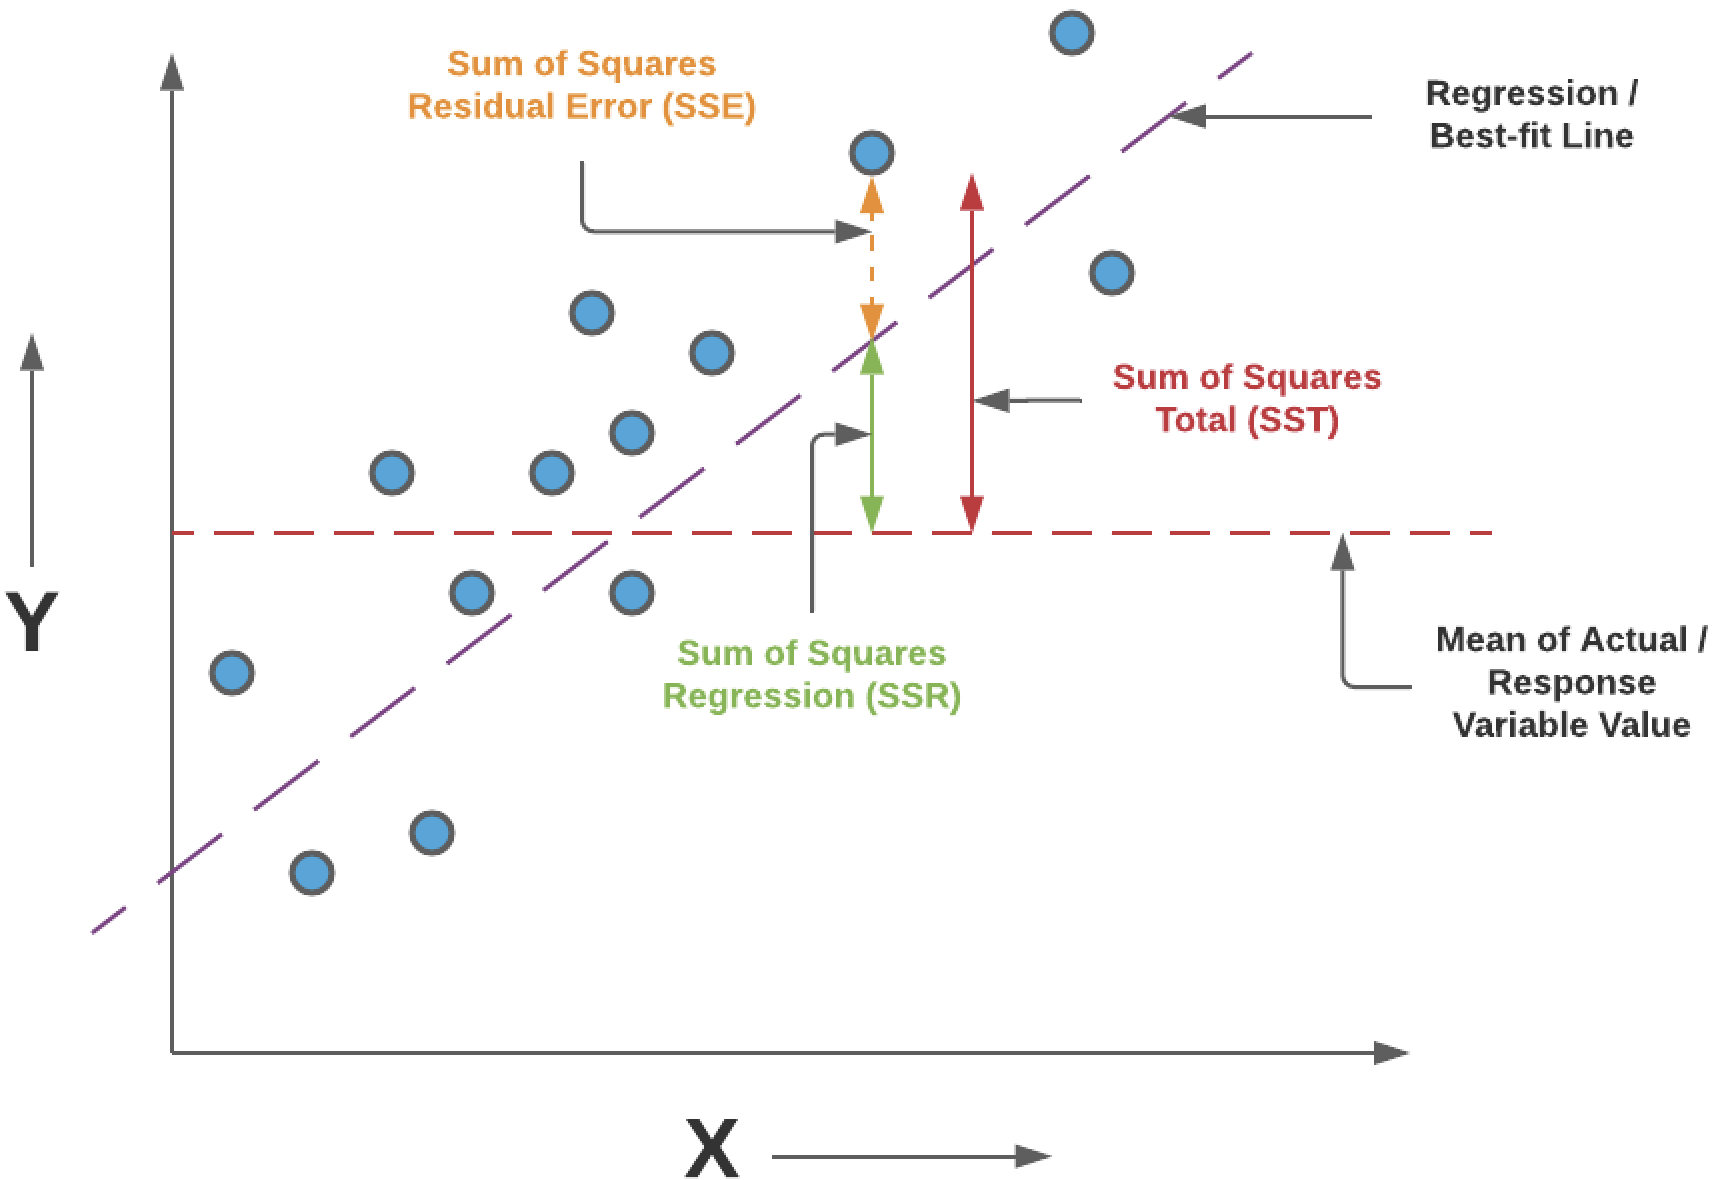
\includegraphics[scale=0.3]{quant/ssr}
\caption{Regression Error Terms}
\end{figure}
 
\begin{definition} \hlt{Error Terminology}
\begin{enumerate}[label=\roman*.]
\setlength{\itemsep}{0pt}
\item Sum of total squares (SST): measures total variation in dependent variable. Sum of squared differences between actual and mean value, $SST = \sum\limits_{i=1}^n (Y_i - \overline{Y})^2 = SSR + SSE$.
\item Sum of squares regression (SSR): measures variation in dependent variable as explained by independent variable. Sum of square distances between predicted and mean value, $SSR = \sum\limits_{i=1}^n (\hat{Y}_i - \overline{Y})^2$.
\item Sum of squares residual error (SSE): measures unexplained variation in dependent variable. Sum of squared vertical distance between actual and predicted values. $SSE = \sum\limits_{i=1}^n (Y_i - \hat{Y})^2$.
\item Mean squares regression (MSR): $MSR = \frac{SSR}{k}$, where $k$ is number of independent variables.
\item Mean squares error (MSE): $MSE = \frac{SSE}{n-k-1}$, where $k$ is number of independent variables.
\item Standard error of estimate (SEE): $SEE = \sqrt{\frac{\sum\limits_{i=1}^n (Y_i - \hat{Y})}{n-2}} = \sqrt{MSE}$.
\item Standard error of intercept: $SE_{\hat{b}_0} = \sqrt{\frac{1}{n} + \frac{\overline{X}^2}{\sum\limits_{i=1}^n(X_i - \overline{X})^2}}$
\end{enumerate}
\end{definition}

\begin{definition} \hlt{Test of Slope Coefficient Significance}
\begin{enumerate}[label=\arabic*.]
\setlength{\itemsep}{0pt}
\item State the hypothesis: $H_0: b_1 = 0$ versus $H_{\alpha} : b_1 \neq 0$
\item Identify the appropriate test statistic:
\begin{align}
t &= \frac{\hat{b}_1 - b_1}{SE_{\hat{b}_1}}, \ \ \ SE_{\hat{b}_1} = \frac{SE}{\sqrt{{\sum\limits_{i=1}^n (X_i - \overline{X})^2}}} \nonumber
\end{align}
with $df = n-2$, where $n$ is number of observations, $SE$ is model standard error of estimate.
\item Specify level of significance $\alpha \%$, for two-side test
\item State the decision rule: Reject $H_0$ if calculated $t$-statistic $>$ critical $t_{\alpha/2}$-value or $<$ $-$ critical $t_{\alpha/2}$-value
\end{enumerate}
\end{definition}

\begin{definition} \hlt{Test of Slope Intercept Significance}
\begin{enumerate}[label=\arabic*.]
\setlength{\itemsep}{0pt}
\item State the hypothesis: $H_0: b_0 \leq B_0$ versus $H_{\alpha} : b_0 > B_0$
\item Identify the appropriate test statistic:
\begin{equation}
t = \frac{\hat{b}_0 - B_0}{SE_{\hat{b}_0}} = \frac{\hat{b}_0 - B_0}{\sqrt{\frac{1}{n} + \frac{\overline{X}^2}{\sum\limits_{i=1}^n (X_i - \overline{X})^2}}} \nonumber
\end{equation}
with $df = n-2$, where $n$ is number of observations.
\item Specify level of significance $\alpha \%$, for two-side test
\item State the decision rule: Reject $H_0$ if calculated $t$-statistic $>$ critical $t_{\alpha/2}$-value or $<$ $-$ critical $t_{\alpha/2}$-value
\end{enumerate}
\end{definition}

\begin{definition} \hlt{Standard Error of Forecast}\\
Interval estimate of forecast, computed as
\begin{equation}
s_f = SE \sqrt{1 + \frac{1}{n} + \frac{(X_f - \overline{X})^2}{\sum\limits_{i=1}^n (X_i - \overline{X})^2}} \nonumber
\end{equation}
where $SE$ is standard error of estimate, $m$ is number of observations, $X_f$ is forecasted value of independent variable, $\overline{X}$ is estimated mean.
\end{definition}

\begin{definition} \hlt{Coefficient of determination, $R^2$}, measure goodness of fit of regression to data.
\begin{equation}
R^2 = \frac{SST - SSE}{SST} = \frac{SSR}{SST} \nonumber
\end{equation}
\end{definition}

Note that $R^2$ do not allow us to know if coefficients are statistically significant. There is no info on bias in estimated coefficients and predicted values. There is no info if model fit is good as well.

\begin{definition} \hlt{Adjusted $R^2$}, adjusts for degrees of freedom.
\begin{equation}
\overline{R}^2 = 1 - \left[\left(\frac{n-1}{n-k-1} \right) (1-R^2) \right] \nonumber
\end{equation}
where $k$ is number of independent variables.
\end{definition}

If we are adding new independent variable to the regression, if the coefficient t-statistics $> \abs{1.0}$, then $\overline{R}^2$ will increase. If coefficient t-statistics $< \abs{1.0}$, then $\overline{R}^2$ will decrease.

\begin{definition} \hlt{Information Criterions}
\begin{enumerate}[label=\roman*.]
\setlength{\itemsep}{0pt}
\item \hlt{Akaike Information Criterion (AIC)}: evaluate model parsimony. Lower AIC means better fitting.
\begin{equation}
AIC = n \ln(\frac{SSE}{n}) + 2(k+1) \nonumber
\end{equation}
where $n$ is the sample size, k is number of independent variables.
\item \hlt{Bayesian Information Criterion (BIC)}: gives greater penalty than AIC if model has more parameters. Lower BIC means better fitting.
\begin{equation}
BIC = n \ln(\frac{SSE}{n}) + \ln(n)(k+1) \nonumber
\end{equation}
\end{enumerate}
\end{definition}

AIC is preferred if model is used for prediction. BIC is preferred if best goodness of fit is desired.

\begin{definition} \hlt{Analysis of Variance (ANOVA)}\\
Analyses the total variability of the dependent variable. The goodness of fit test for whole model is:
\begin{enumerate}[label=\arabic*.]
\setlength{\itemsep}{0pt}
\item State the hypothesis: $H_0 = b_1 = \cdots = b_k = 0$ versus $H_a:$ at least one $b_j \neq 0$
\item Identify the appropriate test statistic: $F = \frac{MSR}{MSE}$, with $df = (k, n-k-1)$\\
where $k$ is number of independent variables, $n$ is number of observations.
\item Specify level of significance $\alpha \%$, for one-side right-tail test
\item State the decision rule: Reject the null if calculated $F$-statistic $>$ critical $F$-value
\end{enumerate}
For restricted versus unrestricted model, the test statistic used is $F = \frac{(SSE_R - SSE_U)/q}{SSE_U/(n-k-1)}$, where $SSE_R$ and $SSE_U$ is $SSE$ of restricted and unrestricted model, $q$ is number of excluded variables in restricted model
\end{definition}

\begin{flushleft}
ANOVA Table
\begin{tabularx}{\textwidth}{p{5em}|p{10em}|p{3em}|p{10em}|X}
\hline
\rowcolor{gray!30}
Source & Sum of Squares & $df$ & Mean Square & $F$-Statistics \\
\hline
Regression & $SSR = \sum\limits_{i=1}^n (\hat{Y}_i - \overline{Y})^2$ & $1$ & $MSR = \frac{SSR}{1}$ & $F = \frac{MSR}{MSE}$\\
Error & $SSE = \sum\limits_{i=1}^n (Y_i - \hat{Y})^2$ & $n-2$ & $MSE = \frac{SSE}{n-2} = SE^2$ & \\
Total & $SST = \sum\limits_{i=1}^n (Y_i - \overline{Y})^2$ & $n-1$ & & \\
\hline
\end{tabularx}
\end{flushleft}

\begin{flushleft}
Assessing model fit using multiple regression statistics
\begin{tabularx}{\textwidth}{p{18em}|X}
\hline
\rowcolor{gray!30}
Statistic & Criterion to use in assessment \\
\hline
Adjusted $R^2$ & The higher the better \\
AIC & The lower the better \\
BIC & The lower the better \\
$t$-statistic on slope coefficient & Outside bounds of critical $t$-values for selected significance level\\
$F$-test for joint test of slope coefficients & Exceeds critical $F$-value for selected significance level\\
\hline
\end{tabularx}
\end{flushleft}

\begin{flushleft}
Principles for proper regression model specification
\begin{tabularx}{\textwidth}{p{18em}|X}
\hline
\rowcolor{gray!30}
Principle & Explanation\\
\hline
Grounded in economic reasoning & Provide economic reasoning behind choice of variables\\
Parsimonious & Each variable play essential role\\
Perform well out of sample & Ensure model is not overfitted\\
Functional form is appropriate & Model to incorporate appropriate nonlinear terms if any\\
Satisfy regression assumptions & Ensure no heteroskedasticity, serial correlation, multicollinearity\\
\hline
\end{tabularx}
\end{flushleft}

\begin{flushleft}
Failures in regression functional form
\begin{tabularx}{\textwidth}{p{14em}|p{15em}|X}
\hline
\rowcolor{gray!30}
Failure & Details & Consequence \\
\hline
Omitted variables & Important variables omitted & Heteroskedasticity, serial correlation\\
Inappropriate form of variables & Non-linear relationship ignored & Heteroskedasticity\\
Inappropriate variable scaling & Variable to be transformed first & Heteroskedasticity, multicollinearity\\
Inappropriate data pooling & Data from different samples pooled & Heteroskedasticity, serial correlation\\
\hline
\end{tabularx}
\end{flushleft}

\newpage

\begin{flushleft}
Summary of violations of assumptions from model misspecification. Let $SE$ be standard errors.
\begin{tabularx}{\textwidth}{p{8em}|X|p{10em}|X}
\hline
\rowcolor{gray!30}
Violation & Issue & Detection & Correction \\
\hline
Heteroskedasticity & Biased coefficient $SE$ & Visual inspection of residuals; BP Test & Revised model, use robust $SE$\\
\hline
Serial Correlation & Inconsistent estimates of coefficients, biased $SE$ & BG Test & Revised model, use serial correlation consistent $SE$\\
\hline
Multicollinearity & Inflated $SE$ & VIF & Revised model; $\uparrow$ sample size \\
\hline
\end{tabularx}
\end{flushleft}

\subsubsection{Heteroskedasticity}

\begin{remark} \hlt{Types of Heteroskedasticity}
\begin{enumerate}[label=\roman*.]
\setlength{\itemsep}{0pt}
\item Unconditional Heteroskedasticity: error variance uncorrelated with value of independent variable.\\
Violates equal variance assumption, but does not cause major problem for regression.
\item Conditional Heteroskedasticity: error variance conditional on value of independent variables.\\
Creates significant problems for statistical inference.\\
MSE is biased estimator of true population variance (error usually underestimated, Type I errors).\\
$F$-test for the overall model is unreliable.
\end{enumerate}
\end{remark}

\begin{figure}[H]
\centering
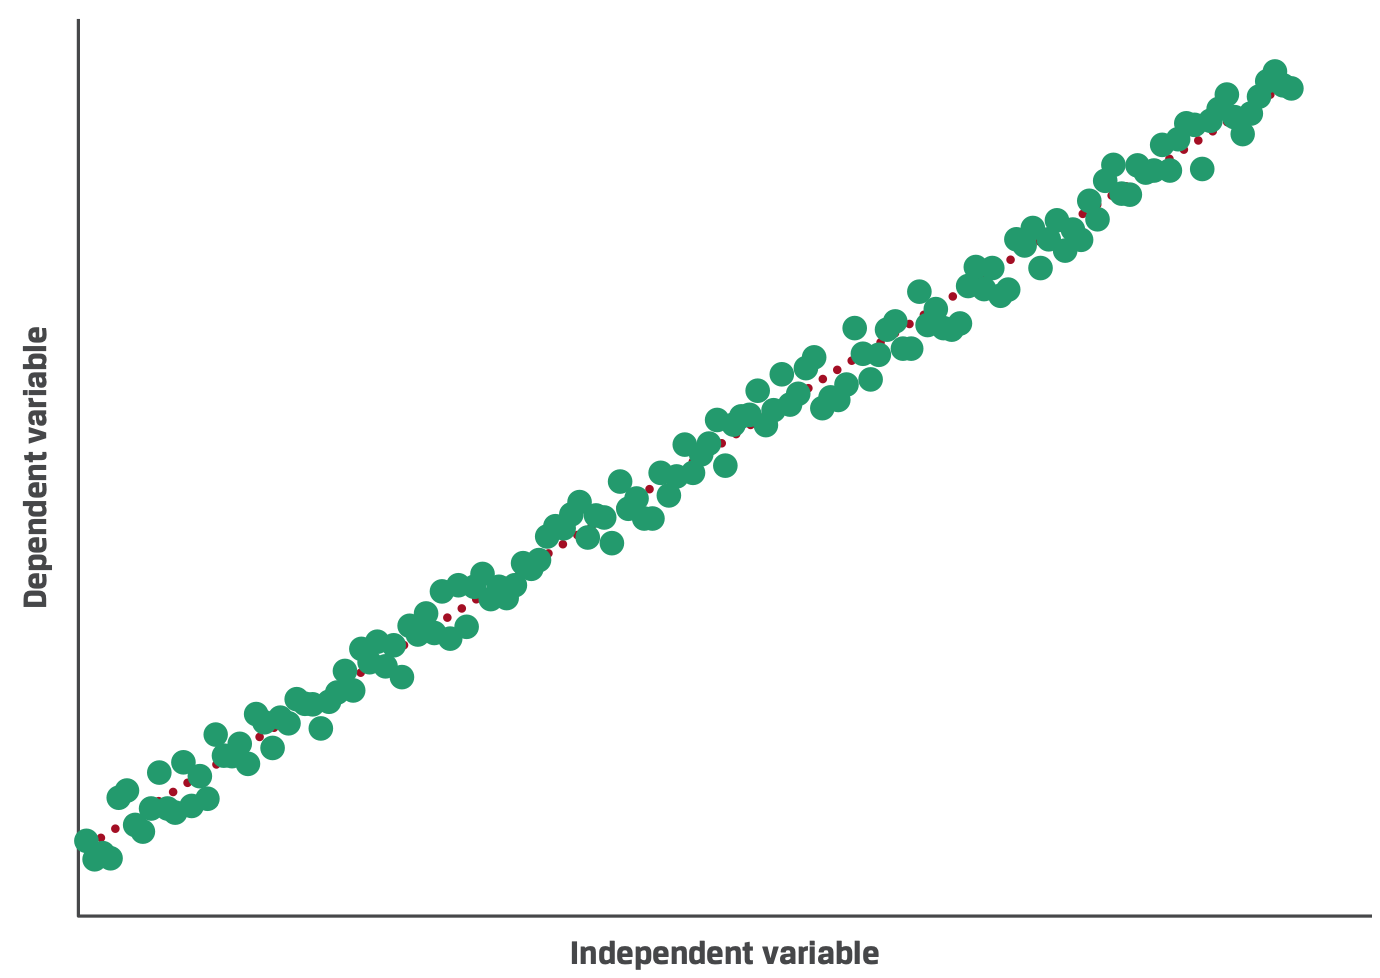
\includegraphics[scale=0.26]{/quant/homoske}
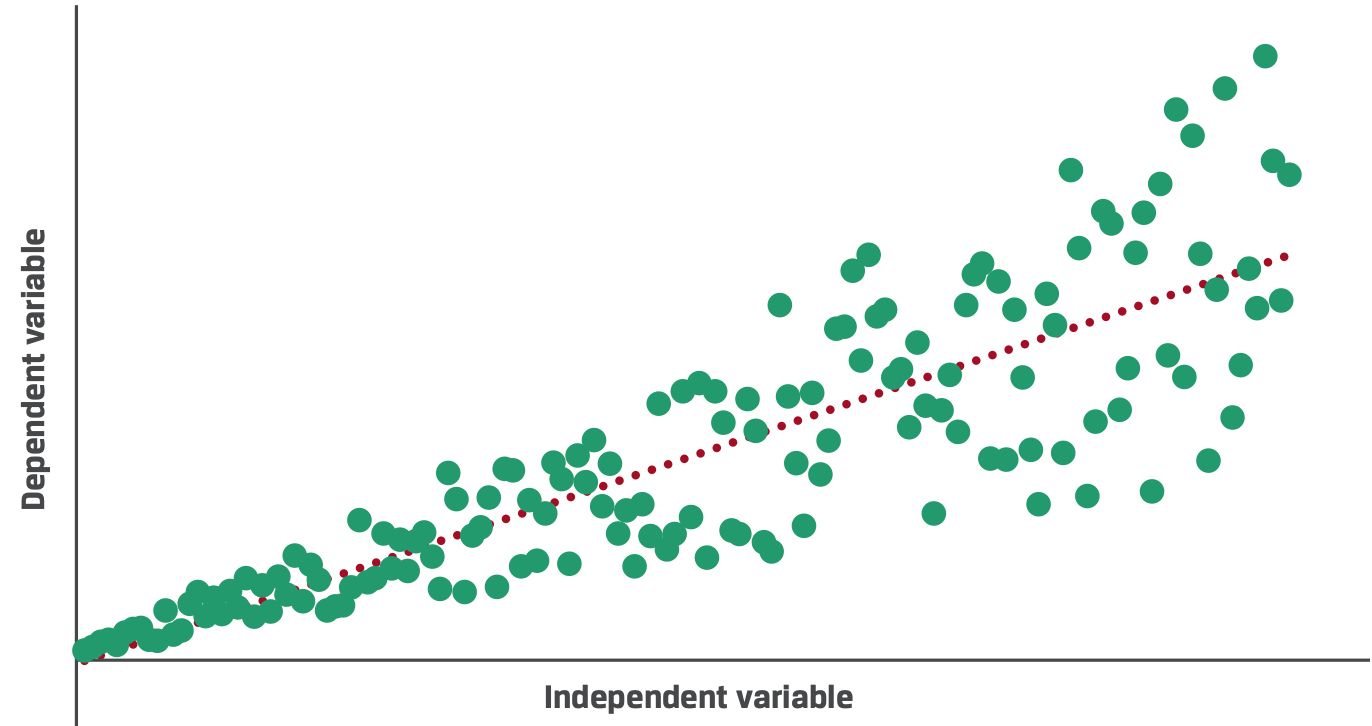
\includegraphics[scale=0.35]{/quant/heteroske}
\caption{Homoskedastic residuals versus heteroskedastic residuals}
\end{figure}

\begin{definition} \hlt{Breusch-Pagan (BP) Test for Conditional Heteroskedastic}
\begin{enumerate}[label=\arabic*.]
\setlength{\itemsep}{0pt}
\item Run the initial regression
\begin{equation}
Y_0 = b_0 + \sum\limits_{i=1}^n b_{i} X_{it} + u_t \nonumber
\end{equation}
\item Run new model with fitted residuals squared from Step 1 as the dependent variable against the regressors.
\begin{equation}
\hat{u}_{t}^2 = a_0 + \sum\limits_{i=1}^n a_{i} X_{it} + \epsilon_t \nonumber
\end{equation}
\item Test the hypothesis on coefficients of the regressors in Step 2 using a $\chi^2$ distributed test statistic
\begin{enumerate}[label=\roman*.]
\setlength{\itemsep}{0pt}
\item State the hypothesis: $H_0:$ all $a_i = 0$ versus $H_{\alpha}:$ at least one $a_i \neq 0$
\item Identify the appropriate test statistic:
\begin{align}
\chi^2_{BP, k} = nR^2 \nonumber
\end{align}
with $df = k$ the number of independent variables in Step 1, $R^2$ is from Step 2, $n$ $\#$ of observations
\item Specify level of significance $\alpha \%$, for one-tail right-sided test
\item State the decision rule: Reject $H_0$ if calculated $\chi^2$-statistic $>$ critical $\chi^2$-value
\end{enumerate}
\end{enumerate}
\end{definition}

\begin{remark} \hlt{Correcting for Heteroskedasticity}\\
Compute robust standard errors, which adjust the standard errors of the regression’s estimated coefficients to account for the heteroskedasticity. The robust standard errors are also known as heteroskedasticity-consistent standard errors or White-corrected standard errors. These robust standard errors are then used to recalculate the $t$-statistics using the original regression coefficients for hypothesis testing.
\end{remark}

\subsubsection{Serial Correlation}

\begin{definition} \hlt{Serial Correlation}\\
Regression residual terms are correlated with one another.
\begin{enumerate}[label=\roman*.]
\setlength{\itemsep}{0pt}
\item Positive Autocorrelation: positive residual at $t-1$ $\uparrow$ probability of observing positive residual at $t$
\item Negative Autocorrelation: positive residual at $t-1$ $\uparrow$ probability of observing negative residual at $t$
\end{enumerate}
\end{definition}

\begin{remark} \hlt{Effects of Serial Correlation}\\
Positive serial correlation results in coefficient standard errors that are too small, causing the computed $t$-statistics and $F$-statistics to be larger, leading to Type I errors. Estimates of slope coefficients inconsistent.
\end{remark}

\begin{definition} \hlt{Durbin-Watson (DW) Test for Autocorrelation}
\begin{equation}
DW = \left[ \sum\limits_{t=2}^T (\epsilon_t - \epsilon_{t-1})^2 \right] / \left[ \sum\limits_{t=1}^T \epsilon_t^2 \right] \nonumber
\end{equation}
$DW = 2:$ indicates there is no autocorrelation detected in the sample.\\
$0 \leq DW < 2:$ point to positive autocorrelation.\\
$2 < DW \leq 4:$ point to negative autocorrelation.
\end{definition}

\begin{definition} \hlt{Breusch–Godfrey (BG) Test for Autocorrelation}
\begin{enumerate}[label=\arabic*.]
\setlength{\itemsep}{0pt}
\item Run the initial regression
\begin{equation}
Y_0 = b_0 + \sum\limits_{i=1}^n b_{i} X_{it} + u_t \nonumber
\end{equation}
\item Run new model with fitted residuals from Step 1 against initial regressors and lagged residuals.
\begin{equation}
\hat{u}_{t} = a_0 + \sum\limits_{i=1}^n a_{i} X_{it} + \sum\limits_{j=1}^m p_j u_{t-j} + \epsilon_t \nonumber
\end{equation}
\item Test the hypothesis on coefficients of the regressors in Step 2 using $\chi^2$ or $F$ test statistic
\begin{enumerate}[label=\roman*.]
\setlength{\itemsep}{0pt}
\item State the hypothesis: $H_0: p_j = 0$ versus $H_{\alpha}: p_j \neq 0$
\item Identify the appropriate test statistic: $F$-distribution with $df = (p, n-p-k-1)$, where $p$ is number of lags tested
\item Specify level of significance $\alpha \%$, for one-tail right-sided test
\item State the decision rule: Reject $H_0$ if calculated $F$-statistic $>$ critical $F$-value
\end{enumerate}
\end{enumerate}
\end{definition}

\begin{remark} \hlt{Correcting for Serial Correlation}\\
Compute robust standard errors (also known as serial-correlation consistent standard errors, serial correlation and heteroskedasticity adjusted standard errors, Newey–West standard errors). These robust standard errors also corrects for conditional heteroskedasticity. These robust standard errors are then used to recalculate the $t$-statistics using the original regression coefficients for hypothesis testing.
\end{remark}

\subsubsection{Multicollinearity}

\begin{remark} \hlt{Effects of Multicollinearity}\\
Condition where two or more independent variables are highly correlated with each other.\\
Inflates standard errors, high $R^2$, significant $F$-statistics, but lowers $t$-statistic. Estimates of slope coefficients imprecise and unreliable. Leads to more Type II errors, as precise credit cannot be assigned to error variation.
\end{remark}

\begin{definition} \hlt{Variance Inflation Factor (VIF) Test for Multicollinearity}\\
$F$-test indicates model is significant, $R^2$ is high, but none of coefficient $t$-tests are significantly different from $0$.
\begin{enumerate}[label=\roman*.]
\setlength{\itemsep}{0pt}
\item Regress one of the independent variable $X_j$ against remaining $k-1$ independent variables.
\item Compute $VIF_j = \frac{1}{R^2_j}$ where $R^2_j$ is from the regression model earlier.
\end{enumerate}
Note, $VIF \geq 1$. If $VIF = 1$, variable $j$ is not highly correlated with other independent variables.\\
$VIF < 5$ indicates further investigation needed, $VIF > 10$ indicates severe multicollinearity.
\end{definition}

\begin{remark} \hlt{Correcting for Multicollinearity}
\begin{enumerate}[label=\roman*.]
\setlength{\itemsep}{0pt}
\item Excluding one or more of the regression variables
\item Using a different proxy for one of the variables
\item Increasing the sample size
\end{enumerate}
\end{remark}

\subsubsection{Influence Analysis}

\begin{definition} \hlt{Types of Outliers}\\
Outliers are extreme observations of the dependent variable.\\
High leverage points are extreme observations of the independent variable.
\end{definition}

\begin{figure}[H]
\centering
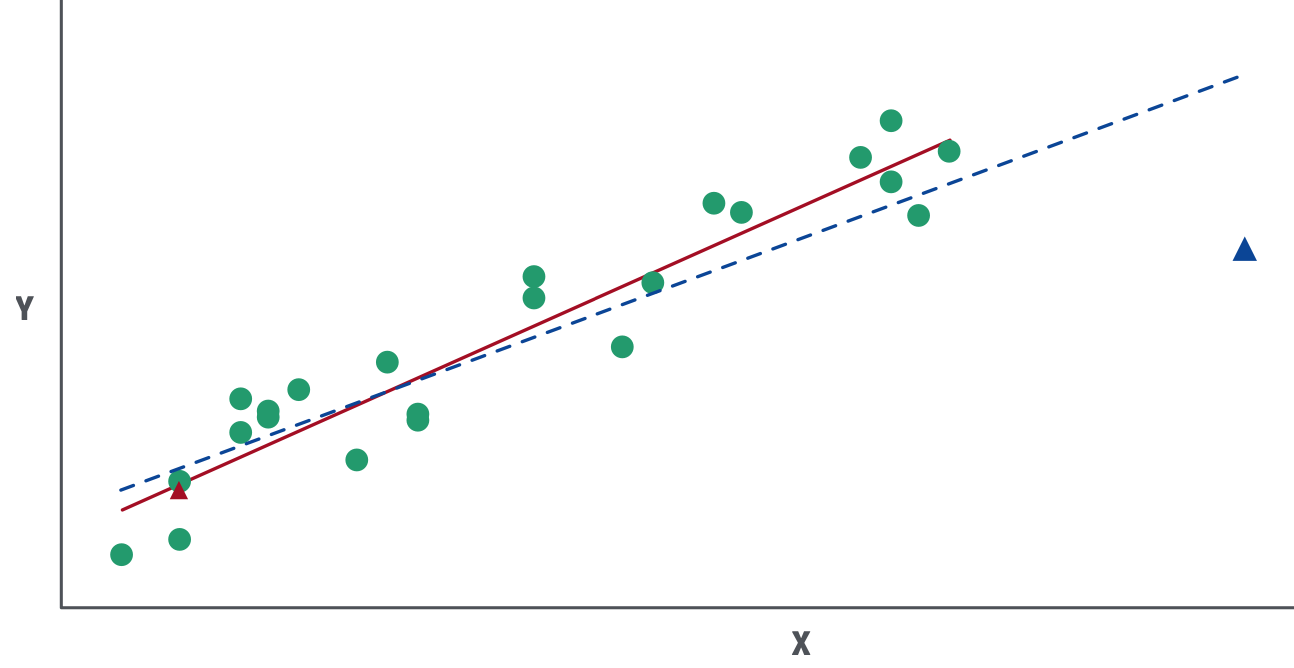
\includegraphics[scale=0.33]{/quant/highlevpoint}
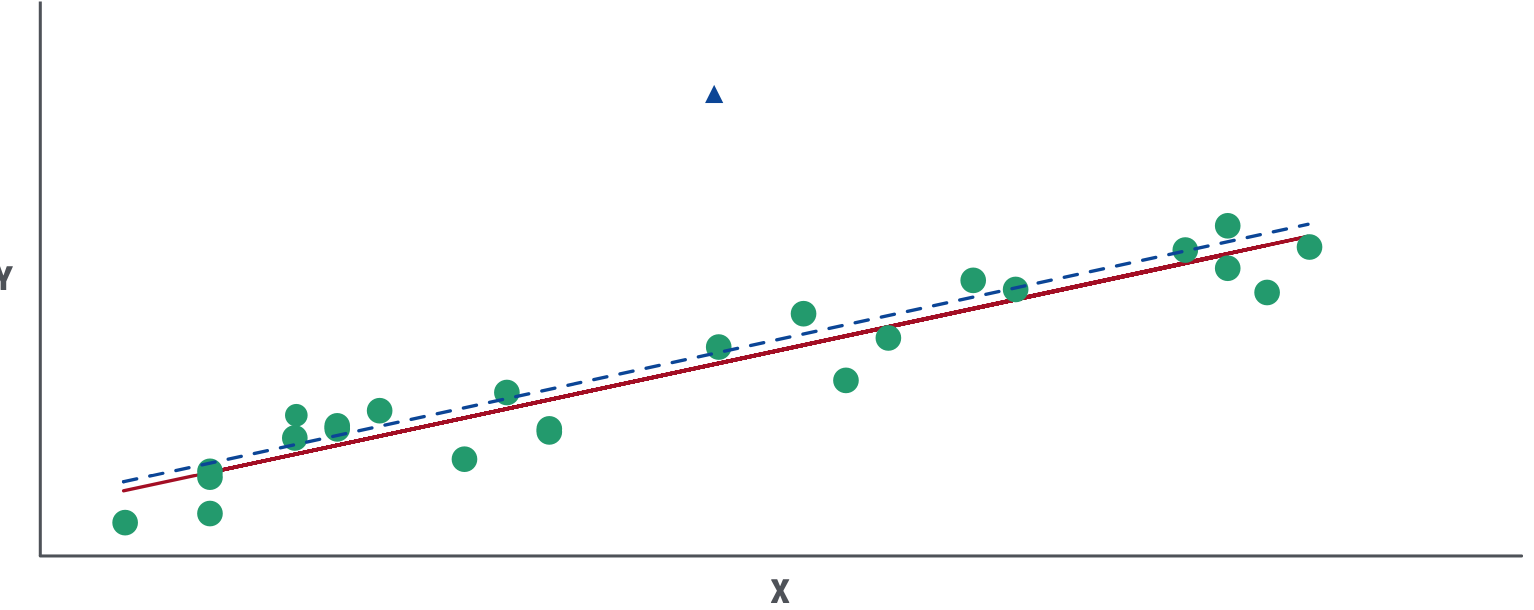
\includegraphics[scale=0.34]{/quant/outlier}
\caption{High-leverage point, and outlier}
\end{figure}

\begin{remark} \hlt{Leverage to Detect Leverage Points}\\
Leverage $0 \leq h_{ii} \leq 1$ is a measure of distance between $j$th observation of independent variable $i$ relative to its sample mean. The higher the value of leverage, the greater the distance, and hence the higher the potential influence of the observation on estimated regression parameters.\\
The sum of individual leverages for all observations is $k+1$, where $k$ is number of independent variables.\\
If variable leverage $h_{ii} > 3 \left( \frac{k+1}{n} \right)$, it is considered potentially influential.
\end{remark}

\begin{remark} \hlt{Studentised Residuals for Outlier}
\begin{enumerate}[label=\roman*.]
\setlength{\itemsep}{0pt}
\item Estimate initial model with $n$ observations, then sequentially delete observations one at a time, and each time re-estimate the model on remaining $(n-1)$ observations.
\item Compare observed $Y$ values (on n observations) with predicted $\hat{Y}$ from models with $i$th observation deleted on $(n-1)$ observations. For given $i$, the residual is then $e^{*}_i = Y_i - \hat{Y}_i^{*}$
\item Divide this residual by standard error of residuals, which produces the studentised deleted residual
\begin{equation}
t_{i^*} = \frac{e^{*}_i}{s_{e^*}} = \frac{e_i}{\sqrt{MSE_{(i)} (1-h_{ii})}} \nonumber
\end{equation}
where $e^{*}_i$ is residual with $i$th observation deleted, $s_{e^*}$ is s.d. of all residuals, $k$ is number of independent variables, $MSE_{(i)}$ is MSE of regression model that deletes $i$th observation, $h_{ii}$ is $i$th observation leverage.\\
If $\abs{t_{i^*}} > 3$, flag observation as outlier.\\
If $\abs{t_{i^*}} >$ critical value of $t$-statistic with $df=n-k-2$ at selected significance level, potential influential
\end{enumerate}
\end{remark}

\begin{remark} \hlt{Cook's Distance Test of Influential Data Points}\\
Outliers and high-leverage points are not necessarily influential.\\
Observation is influential if exclusion from sample causes substantial changes in estimated regression function.
\begin{equation}
D_i = \frac{e_i^2}{(k+1)MSE} \left[ \frac{h_{ii}}{(1-h_{ii})^2} \right] \nonumber
\end{equation}
where $e_i$ is residual for observation $i$.\\
Cook's distance is distributed as an $F$-distribution with $df = (k+1, n-k-1)$.\\
If $D_i \geq 0.5$, observation may be influential and merits further investigation.\\
If $D_i \geq 1$ or $D_i \geq \sqrt{k/n}$, observation is highly likely to be an influential datapoint.
\end{remark}

\begin{remark} \hlt{Key Points on Cook's Distance}
\begin{enumerate}[label=\roman*.]
\setlength{\itemsep}{0pt}
\item $D_i$ depends on both residuals and leverages, so it is a composite measure.
\item $D_i$ summarises in a single measure how much all of the regression’s estimated values change when $i$th observation is deleted from the sample.
\item A large $D_i$ indicates that the $i$th observation strongly influences the regression’s estimated values.
\end{enumerate}
\end{remark}

\begin{figure}[H]
\centering
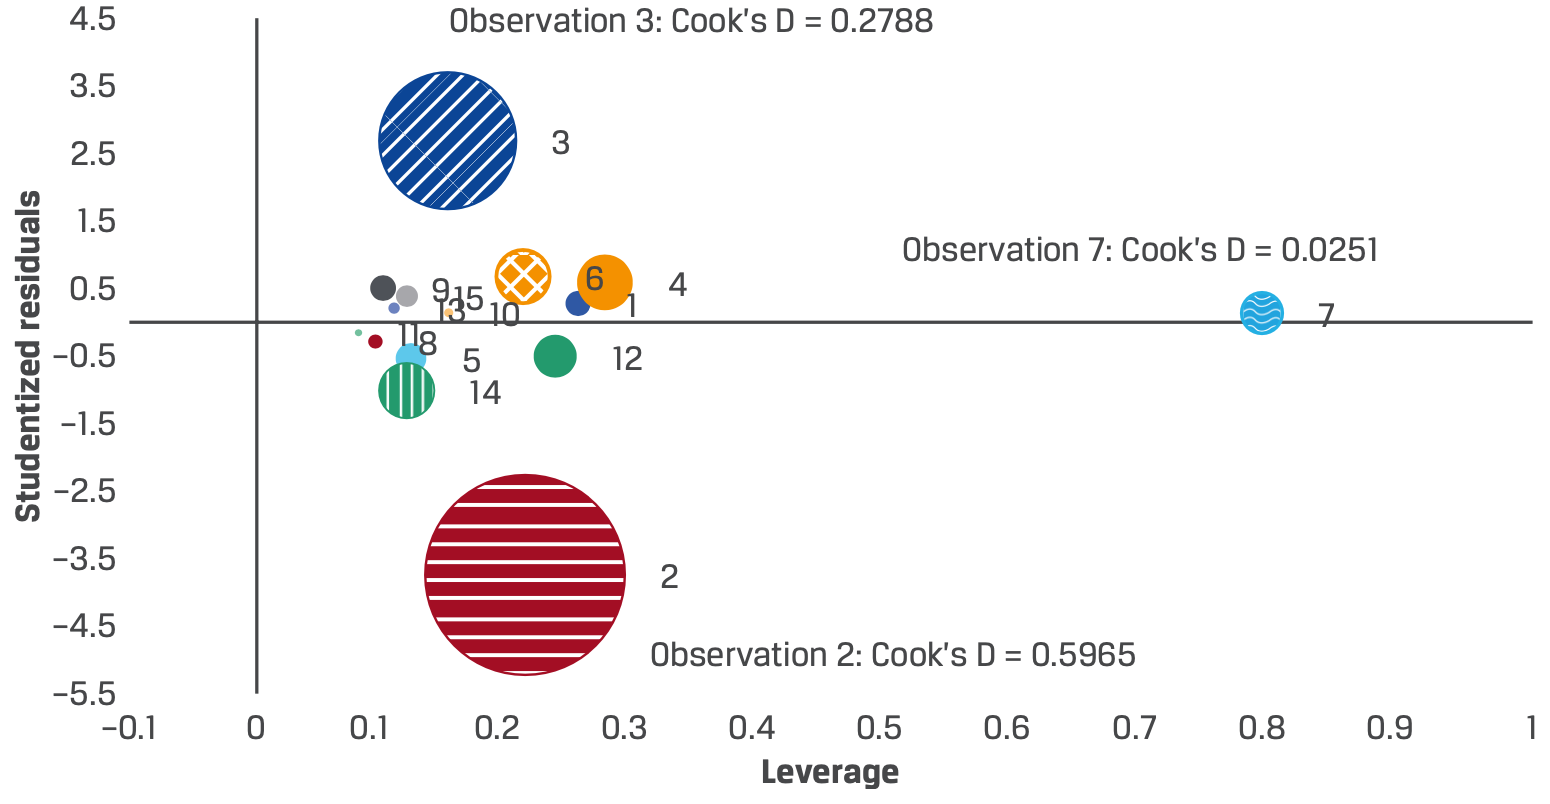
\includegraphics[scale=0.45]{/quant/influplot}
\caption{Example of influence plot}
\end{figure}

\begin{flushleft}
Summary of Measures of Influential Observations
\begin{tabularx}{\textwidth}{p{11em}|p{2.8em}|p{2.8em}|p{16em}|X}
\hline
\rowcolor{gray!30}
Measure & $Y$-Var & $X$-Var & Process & Criteria as Influential\\
\hline
Leverage $h_{ii}$ & & \checkmark & $0 \leq h_{ii} \leq 1$ & $h_{ii} > 3 \left( \frac{k+1}{n} \right)$ \\
Studentised residual $t_{i^*}$ & \checkmark & & Compare with $t$-stat, $df = n-k-2$ & $\abs{t_{i^*}} > 3$, $\abs{t_{i^*}} > t_{\alpha}$ \\
Cook's Distance $D_i$ & \checkmark & \checkmark & Compare with $\sqrt{k/n}$ & $D_i \geq 1$, $D_i \geq \sqrt{k/n}$ \\
\hline 
\end{tabularx}
\end{flushleft}

\begin{remark} \hlt{Types of Dummy Variables}\\
Note, $n$ categories require $n-1$ dummy variables, where $D_i \in \{0, 1\}$.
\begin{enumerate}[label=\roman*.]
\setlength{\itemsep}{0pt}
\item Intercept dummy $D$ with constant $d_0$, model is then $Y_i = b_0 + d_0 D + b_1 X_i + \epsilon_i$
\item Slope dummy $D$ with variable $X_i$, model is then $Y_i = b_0 + b_1 X_i + d_1 D_i X_i + \epsilon_i$
\end{enumerate}
\end{remark}

\begin{figure}[H]
\centering
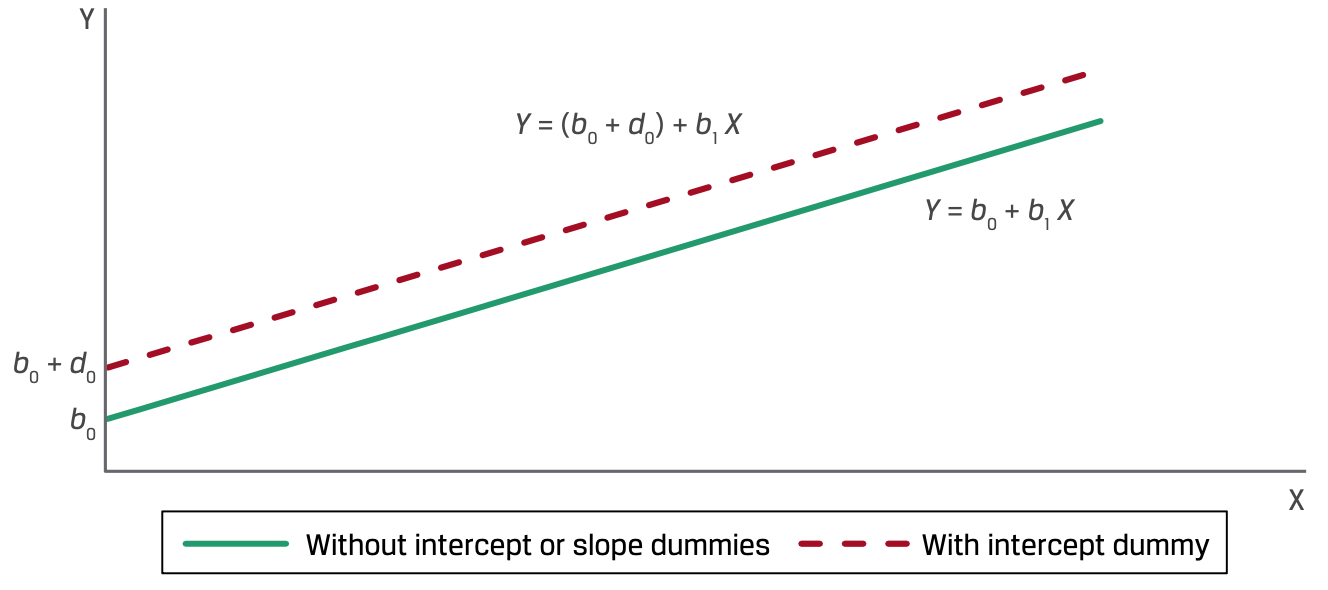
\includegraphics[scale=0.35]{/quant/intercept}
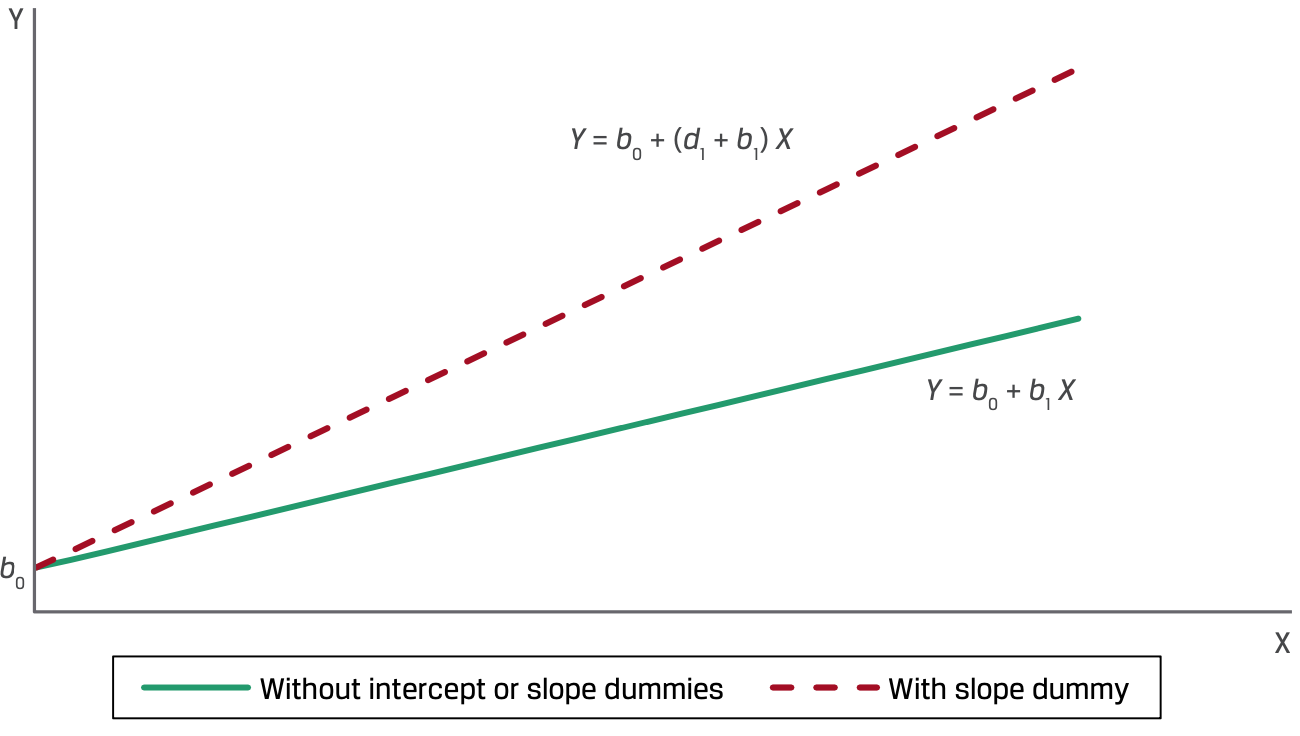
\includegraphics[scale=0.35]{/quant/slope}
\caption{Intercept dummy variable and slope dummy variable}
\end{figure}

\begin{definition} \hlt{Logistic Regression}\\
Provides outcome variable (qualitative dependent variable) describing data that fit into categories, $Y \in \{0, 1\}$.
\begin{equation}
\ln \left( \frac{p}{1-p} \right) = b_0 + \sum\limits_{i=1}^n b_i X_i + \epsilon \nonumber
\end{equation}
where $\ln \left( \frac{p}{1-p} \right)$ is $\log$ likelihood.\\
Regression coefficients are estimated with maximum likelihood estimation (MLE).\\
Pseudo-$R^2$ is used to compare different specifications of the same model (model based on same datasets).
\end{definition}

\begin{definition} \hlt{Likelihood Ratio Test}\\
Method to assess the fit of logistic regression models and is based on the log-likelihood metric.
\begin{equation}
LR = -2 \times (\log l_{R} - \log l_{U}) \nonumber
\end{equation}
where $\log l_{R}, \log l_{U}$ are log-likelihood of restricted and unrestricted models.
$LR$ distributed as $\chi^2$ with $df = q$, where $q$ is number of restrictions. Higher $LR$ is better.
\end{definition}